\documentclass[11pt]{article}
\usepackage[a3paper,landscape,margin=15mm]{geometry}

\usepackage{fontspec}
\setmainfont{Nimbus Roman}
\setsansfont{Nimbus Sans}
\setmonofont{Nimbus Mono PS}
\usepackage[authoryear]{natbib}
\usepackage{amsmath,amssymb,graphicx,booktabs,array,xcolor,caption,tikz,longtable}
\usetikzlibrary{positioning,fit,arrows.meta}
\usepackage{microtype}
\microtypesetup{expansion=false}
\usepackage{url}
\setlength{\emergencystretch}{3em}
\setlength{\parindent}{0pt}
\setlength{\parskip}{4pt}
\newcommand{\ibar}{\bar{y}}
\newcommand{\sbar}{\bar{s}}
\newcommand{\Exp}{\mathrm{Exp}}
\newcommand{\Full}{\textup{\textsc{Full}}}
\newcommand{\TS}{\textup{\textsc{TwoScale}}}
\newcommand{\ind}{\mathbf{1}}
\newcommand{\eW}{e_W}

\begin{document}
\begin{center}\Large Розділи 1--3: простіша українська редакція\end{center}
Відповідні фрагменти вирівняно поруч. Нумерація розділів, формул і посилань відповідає вихідній статті.
\setlength{\tabcolsep}{6mm}
\begin{longtable}{@{}p{0.475\textwidth}|p{0.475\textwidth}@{}}
\Large\textbf{До} & \Large\textbf{Після}\\\hline\endhead
\begin{minipage}[t]{\linewidth}
\section*{1. Вступ}
\end{minipage} &
\begin{minipage}[t]{\linewidth}
\section*{1. Вступ}
\end{minipage} \\[5mm]
\begin{minipage}[t]{\linewidth}
Епідемія поширюється на кількох рівнях. Усередині спільноти зараження може залежати від конкретних контактів між людьми \citep{keeling2005,pastorsatorras2015,kiss2017}. Для зв'язків між спільнотами дані часто менш докладні: наприклад, відома лише кількість пасажирів, обсяг поїздок на роботу або загальна вага зв'язку між двома місцями \citep{balcan2009,barbosa2018human}. Тому потрібна модель, яка поєднує докладну контактну мережу всередині кожної спільноти із загальними даними про зв'язки між спільнотами.
\end{minipage} &
\begin{minipage}[t]{\linewidth}
Інфекція поширюється як усередині спільнот, так і між ними. Усередині спільноти важливо, хто саме з ким контактує \citep{keeling2005,pastorsatorras2015,kiss2017}. Про зв'язки між спільнотами часто відомо менше: наприклад, лише кількість пасажирів або поїздок на роботу \citep{balcan2009,barbosa2018human}. Ми досліджуємо модель, яка зберігає окремі контакти всередині спільнот, а зв'язки між ними описує загальними вагами.
\end{minipage} \\[5mm]
\begin{minipage}[t]{\linewidth}
Така ситуація виникає на практиці. Локальну контактну мережу можна спостерігати, відновлювати або генерувати за відомими характеристиками, зокрема кластеризацією та середньою довжиною найкоротших шляхів \citep{eubank2004,danon2011}. Натомість зв'язки між спільнотами можуть бути відомі лише з транспортних, міграційних даних, даних про поїздки на роботу чи даних мобільних операторів \citep{barbosa2018human,chang2021}. Вони дають загальну силу зв'язку, але не визначають людей, через яких інфекція може перейти між спільнотами. Отже, ми можемо знати вагу зв'язку, не знаючи конкретних вузлів-мостів та їхнього стану.
\end{minipage} &
\begin{minipage}[t]{\linewidth}
Контактні мережі можна будувати за даними про населення, його переміщення та контакти \citep{eubank2004,danon2011}. Зв'язки між спільнотами можна оцінювати за транспортними й міграційними даними або даними мобільних операторів \citep{barbosa2018human,chang2021}. Такі дані показують, наскільки сильно пов'язані дві спільноти, але не завжди вказують конкретних людей, через яких може перейти інфекція. Вузли, що мають контакти з іншою спільнотою, далі називаємо вузлами-мостами.
\end{minipage} \\[5mm]
\begin{minipage}[t]{\linewidth}
Якщо відомі всі контакти, епідемію можна описати неперервним марковським ланцюгом (CTMC) і точно моделювати методом Gillespie \citep{gillespie1977exact,gibson2000}. Є також ефективні методи для часових, великих і розріджених мереж \citep{vestergaard2015,kuryliak2025simulating}. Проте їм усе одно потрібні конкретні контакти, здатні передавати інфекцію. Метапопуляційні моделі використовують загальні потоки між спільнотами, але зазвичай замінюють і докладну локальну мережу кількостями людей у різних станах \citep{colizza2007reaction,colizza2008,balcan2010modeling,ajelli2010}. Наша задача лежить між цими двома випадками: зберегти випадкове поширення між окремими вузлами всередині спільнот, використовуючи лише загальні дані для зв'язків між ними.
\end{minipage} &
\begin{minipage}[t]{\linewidth}
Якщо відомі всі контакти, можна моделювати випадкові зараження методом Gillespie. Він точно відтворює заданий неперервний марковський ланцюг (CTMC) \citep{gillespie1977exact,gibson2000}. Існують також ефективні алгоритми для мереж зі змінними в часі контактами та для мережевого моделювання епідемій \citep{vestergaard2015,kuryliak2025simulating}. Їм потрібні конкретні контакти, через які передається інфекція. Метапопуляційні моделі натомість описують спільноти кількостями людей у різних станах і зв'язують їх загальними потоками \citep{colizza2007reaction,colizza2008,balcan2010modeling,ajelli2010}. Ми поєднуємо ці підходи: моделюємо окремі вузли всередині спільнот і використовуємо загальні ваги для передавання між ними.
\end{minipage} \\[5mm]
\begin{minipage}[t]{\linewidth}
Ідею двомасштабного симулятор представлено в попередній конференційній роботі \citep{kuryliak2025towards}. Для кожної спільноти він запускає окремий локальний симулятор. Макрорівень використовує поточні стани спільнот і ваги зв'язків, щоб генерувати зараження, які надходять з іншої спільноти. У цій статті ми докладно описуємо метод і досліджуємо його похибку. Зокрема, з'ясовуємо, що втрачається, коли справжні міжспільнотні ребра та їхні кінцеві вузли замінено загальною вагою зв'язку, а імпортоване зараження потрапляє на випадково вибраний сприйнятливий вузол.
\end{minipage} &
\begin{minipage}[t]{\linewidth}
Ідею двомасштабного симулятора представлено в попередній конференційній роботі \citep{kuryliak2025towards}. Кожна спільнота має свій локальний симулятор. Спільний планувальник, який називаємо макрорівнем, визначає зараження між спільнотами за їхніми поточними станами та вагами зв'язків. Зараження, що надходить з іншої спільноти, називаємо імпортом інфекції. У цій статті описуємо метод і досліджуємо його похибку: що змінюється, коли замість справжніх міжспільнотних контактів відома лише їхня загальна вага, а імпорт потрапляє на випадково вибраний сприйнятливий вузол?
\end{minipage} \\[5mm]
\begin{minipage}[t]{\linewidth}
Головне питання: коли такого агрегованого зв'язку достатньо для відтворення потрібної нам характеристики повномережевого CTMC? Ми досліджуємо часи прибуття інфекції, їхні розподіли та можливість передавання через справжні контакти. Близькі часи прибуття ще не гарантують фізично можливого передавання: агрегована модель може заразити іншу спільноту до того, як заразиться будь-який справжній вузол-міст у спільноті-джерелі. У контрольованих експериментах ми знаємо повну контактну мережу й використовуємо її як еталон. Двомасштабний симулятор отримує лише локальні мережі та загальні ваги зв'язків. Це перевірка методу, а не калібрування моделі конкретної епідемії.
\end{minipage} &
\begin{minipage}[t]{\linewidth}
Головне питання: коли цього спрощення достатньо, щоб правильно оцінити час поширення інфекції? Ми порівнюємо часи її першого прибуття до спільнот і розподіли цих часів за багатьма запусками. Також перевіряємо, чи могло зараження відбутися через справжні контакти. Близькі часи ще не гарантують можливого шляху передавання: двомасштабна модель може заразити іншу спільноту, поки всі справжні вузли-мости в спільноті-джерелі ще сприйнятливі. Для перевірки ми використовуємо синтетичні мережі, у яких знаємо всі контакти. Повний Gillespie отримує всю мережу, а двомасштабний метод --- лише локальні мережі та загальні ваги міжспільнотних зв'язків.
\end{minipage} \\[5mm]
\begin{minipage}[t]{\linewidth}
Стаття має чотири основні результати.
\begin{enumerate}
\item Ми повністю описуємо двомасштабний симулятор, зокрема синхронізацію локальних симуляторів з глобальним з через фіксовані часові інтервали (Розділ~3, Алгоритм~1).
\item Ми показуємо, що саме моделює ідеальний метод із неперервним часом. Він точний для \emph{сурогатної мережі}: справжні міжспільнотні ребра замінено слабкими зв'язками між усіма парами вузлів зі збереженням загальної ваги (Твердження~1). Далі ми визначаємо джерела похибки та аналізуємо один експорт інфекції (Твердження~2).
\item Ми порівнюємо метод із повномережевим моделюванням Gillespie для одиничних експортів і ланцюгів спільнот. Перестановочні перевірки показують, які відмінності можуть виникнути лише через скінченну кількість запусків (Розділи~5 і~6).
\item Ми пропонуємо емпіричний показник точності для наших тестів. Він порівнює розкид часів зараження всередині спільноти з типовим часом передавання через одне міжспільнотне ребро (Розділ~6.6).
\end{enumerate}
\end{minipage} &
\begin{minipage}[t]{\linewidth}
Стаття має чотири основні результати.
\begin{enumerate}
\item Описуємо, як працює симулятор: кожна спільнота моделюється окремо, а спільний планувальник визначає зараження між ними. Пояснюємо, як він узгоджує локальні симулятори на часових інтервалах фіксованої довжини (Розділ~3, Алгоритм~1).
\item Показуємо, яку мережу метод моделює точно, якщо визначати час кожної події без наближення часовою сіткою. Це \emph{сурогатна мережа}: справжні контакти між двома спільнотами замінено слабкими зв'язками між усіма парами їхніх вузлів зі збереженням загальної ваги (Твердження~1). Пояснюємо джерела похибки цієї заміни. Для одного передавання назовні доводимо, що за випадкового рівномірного розміщення мостів такий метод схильний передавати інфекцію раніше за повний Gillespie; точний зміст цього порівняння наведено в Твердженні~2.
\item Порівнюємо метод із повним Gillespie для одного передавання інфекції назовні та для ланцюгів спільнот. У наших тестах за швидкого поширення всередині спільнот розподіли часу прибуття зазвичай близькі. За повільнішого внутрішнього поширення двомасштабний метод систематично дає раніше прибуття. Випадкове переставляння міток методів у результатах запусків допомагає оцінити, чи можна пояснити відмінності скінченною кількістю запусків (Розділи~5 і~6).
\item Пропонуємо показник, який допомагає пояснити точність у наших тестах. Він порівнює розкид часів зараження всередині спільноти із середнім часом передавання через одне міжспільнотне ребро. За малих значень розподіли часу прибуття зазвичай узгоджуються; за більших метод дає раніше прибуття. Це спостереження для досліджених мереж, а не загальний закон похибки (Розділ~6.6).
\end{enumerate}
\end{minipage} \\[5mm]
\begin{minipage}[t]{\linewidth}
Ми розглядаємо динаміку «сприйнятливий--інфікований» (SI) на статичних синтетичних мережах і використовуємо один фіксований крок синхронізації. Розділ~2 пояснює зв'язок із попередніми методами. Розділ~3 описує симулятор. У Розділі~4 пояснено, яку інформацію агрегований зв'язок зберігає та втрачає. Розділи~5 і~6 містять експерименти та результати. У Розділі~7 обговорено застосування, обчислювальні витрати й обмеження.
\end{minipage} &
\begin{minipage}[t]{\linewidth}
У всіх експериментах вузол після зараження залишається інфікованим: це модель «сприйнятливий--інфікований» (SI). Мережі статичні й синтетичні, а крок синхронізації фіксований. Далі описуємо попередні праці (Розділ~2), метод (Розділ~3) та інформацію, яку він зберігає і втрачає (Розділ~4). Експерименти й результати наведено в Розділах~5 і~6, а застосування та обмеження --- у Розділі~7.
\end{minipage} \\[5mm]
\begin{minipage}[t]{\linewidth}
\section*{2. Пов'язані праці}
\end{minipage} &
\begin{minipage}[t]{\linewidth}
\section*{2. Пов'язані праці}
\end{minipage} \\[5mm]
\begin{minipage}[t]{\linewidth}
\paragraph{Моделювання випадкових подій.}
Прямий метод Gillespie вибирає наступну подію та її час за поточними інтенсивностями подій \citep{gillespie1977exact}. Метод наступної реакції підтримує окремий годинник для кожної можливої події \citep{gibson2000}. Обидва методи точні для CTMC, який вони моделюють. Якщо інтенсивність змінюється з часом, її можна накопичувати до досягнення випадкового порога \citep{ethier1986}. \citet{anderson2007} використав цю ідею для систем зі змінними інтенсивностями та затримками. Наш макрогодинник працює за тією самою ідеєю, але його інтенсивність змінюється разом зі станами локальних епідемій. Мережеві симулятори можуть зменшувати обсяг роботи, оновлюючи лише інтенсивності, на які вплинула остання подія \citep{vestergaard2015,kuryliak2025simulating}. Наші локальні симулятори використовують реалізацію з \citet{kuryliak2025simulating}.
\end{minipage} &
\begin{minipage}[t]{\linewidth}
\paragraph{Моделювання випадкових подій.}
Прямий метод Gillespie визначає час наступної події та вибирає її за поточними інтенсивностями --- величинами, що задають частоту подій \citep{gillespie1977exact}. Метод наступної реакції веде окремий годинник для кожної можливої події \citep{gibson2000}. Обидва точно моделюють заданий CTMC. Якщо інтенсивність змінюється, час події можна визначати, накопичуючи її до випадкового порога \citep{ethier1986}. \citet{anderson2007} застосував цю ідею до систем зі змінними інтенсивностями та затримками. Так само працює наш годинник міжспільнотних заражень. Для ефективного мережевого моделювання використовують, зокрема, часовий алгоритм Gillespie та оновлення лише тих інтенсивностей, які змінила остання подія \citep{vestergaard2015,kuryliak2025simulating}. Наші локальні симулятори використовують реалізацію з \citet{kuryliak2025simulating}.
\end{minipage} \\[5mm]
\begin{minipage}[t]{\linewidth}
Деякі багатомасштабні методи прискорюють моделювання хімічних реакцій, наближено описуючи реакції, що відбуваються значно частіше за інші \citep{haseltine2002,cao2005slow}. Наш метод прибирає іншу інформацію. Він зберігає локальні зараження, але не знає, які саме міжспільнотні ребра зараз здатні передавати інфекцію. Попри цю відмінність, співвідношення швидкостей локального поширення та міжспільнотного передавання допомагає пояснити похибку.
\end{minipage} &
\begin{minipage}[t]{\linewidth}
Багатомасштабні методи для хімічних реакцій можуть наближено описувати швидкі реакції, щоб прискорити моделювання \citep{haseltine2002,cao2005slow}. Наше спрощення стосується контактів: локальні зараження моделюються окремо, але конкретні міжспільнотні ребра невідомі. Співвідношення часу поширення всередині спільноти й часу передавання між спільнотами допомагає пояснити наслідки цього спрощення.
\end{minipage} \\[5mm]
\begin{minipage}[t]{\linewidth}
\paragraph{Моделі з кількома спільнотами.}
Метапопуляційні моделі описують кожну підпопуляцію кількостями людей у різних станах і зв'язують підпопуляції потоками мобільності. Їх використовували для дослідження глобального поширення та умов проникнення інфекції \citep{colizza2007reaction,colizza2008,balcan2009,balcan2010modeling}. Докладні дані мобільності також можна поєднувати з локальними моделями передавання \citep{chang2021}. Агентні моделі, своєю чергою, представляють окремих людей у всій системі \citep{eubank2004,kerr2021}. \citet{ajelli2010} порівняли ці два підходи. Досліджуваний тут метод зберігає окремі вузли та контакти всередині спільноти, але замінює невідомі індивідуальні контакти між спільнотами одним агрегованим стохастичним зв'язком.
\end{minipage} &
\begin{minipage}[t]{\linewidth}
\paragraph{Моделі з кількома спільнотами.}
Метапопуляційні моделі рахують людей у різних станах у кожній спільноті й описують переміщення між спільнотами. Так досліджують глобальне поширення та умови проникнення інфекції \citep{colizza2007reaction,colizza2008,balcan2009,balcan2010modeling}. Дані про переміщення також поєднують із локальними моделями передавання \citep{chang2021}. Агентні моделі описують окремих людей у всій системі \citep{eubank2004,kerr2021}. \citet{ajelli2010} порівняли ці підходи. Наш метод зберігає окремі вузли та контакти всередині спільнот, а зараження між ними визначає за загальними вагами зв'язків і поточними кількостями вузлів у різних станах.
\end{minipage} \\[5mm]
\begin{minipage}[t]{\linewidth}
\paragraph{Два рівні перемішування та спільне моделювання.}
Деякі епідемічні моделі поєднують контакти в малих локальних групах із рівномірним перемішуванням на ширшому рівні \citep{ball1997}. Наша сурогатна мережа має подібну ідею, але рівномірне перемішування діє лише між зв'язаними парами спільнот, а його силу визначає загальна вага зв'язку.
\end{minipage} &
\begin{minipage}[t]{\linewidth}
\paragraph{Два рівні перемішування та спільне моделювання.}
Деякі епідемічні моделі враховують окремі контакти в малих групах, а на ширшому рівні припускають рівномірне перемішування \citep{ball1997}. Подібне припущення має наша сурогатна мережа: між двома зв'язаними спільнотами загальну вагу рівномірно розподілено між усіма парами вузлів.
\end{minipage} \\[5mm]
\begin{minipage}[t]{\linewidth}
Реалізація також має риси спільного моделювання (co-simulation). У ньому окремі симулятори підсистем рухаються вперед за спільною часовою сіткою та обмінюються обмеженим набором даних \citep{gomes2018cosim}. У нас цими підсистемами є локальні симулятори спільнот. Вони передають макрорівню кількості інфікованих і сприйнятливих вузлів. Макрорівень використовує ці дані, щоб згенерувати час міжспільнотного зараження та вибрати спільноту-одержувача й цільовий вузол. Отже, локальні симулятори можуть залишатися «чорними скриньками» для планувальника. У цій реалізації дані, якими вони обмінюються, використовуються для створення випадкових подій зараження.
\end{minipage} &
\begin{minipage}[t]{\linewidth}
Метод також пов'язаний зі спільним моделюванням (co-simulation): окремі симулятори працюють за узгодженими часовими інтервалами й обмінюються даними \citep{gomes2018cosim}. У нас кожен локальний симулятор повідомляє кількості інфікованих і сприйнятливих вузлів. Планувальник використовує їх для визначення часу міжспільнотного зараження та вибору його цілі. Йому не потрібно знати всі внутрішні кроки локальних симуляторів.
\end{minipage} \\[5mm]
\begin{minipage}[t]{\linewidth}
\section*{3. Метод двомасштабного моделювання}
\end{minipage} &
\begin{minipage}[t]{\linewidth}
\section*{3. Метод двомасштабного моделювання}
\end{minipage} \\[5mm]
\begin{minipage}[t]{\linewidth}
В експериментах використано одну реалізацію двомасштабного симулятора, яка узгоджує спільноти за часовою сіткою. Щоб зрозуміти її похибку, ми також розглядаємо процес із тими самими інтенсивностями, але з точним визначенням часу кожної події. Цей теоретичний опис називаємо \emph{ідеальним процесом}. Він дає змогу відокремити похибку заміни мережі від додаткової похибки часової сітки. Ідеальний процес точний для сурогатної мережі, визначеної далі; це не означає точності для початкової фізичної мережі. Нижче пояснимо еталонну модель, доступні дані та кроки реалізованого симулятора.
\end{minipage} &
\begin{minipage}[t]{\linewidth}
Усі експерименти використовують одну реалізацію двомасштабного симулятора. Вона узгоджує локальні симулятори на часових інтервалах фіксованої довжини та наближено визначає час зараження між спільнотами. Для пояснення похибки також розглядаємо теоретичну версію з точним часом кожної події. Далі називаємо її \emph{ідеальним процесом}. Це двомасштабний метод без чисельної похибки часової сітки. Він усе ще використовує усереднені зв'язки між спільнотами, тому точно моделює сурогатну мережу, а загалом не початкову мережу зі справжніми контактами. Нижче описуємо обидві мережі та роботу симулятора.
\end{minipage} \\[5mm]
\begin{minipage}[t]{\linewidth}
\subsection*{3.1. Повномережева еталонна модель}
\end{minipage} &
\begin{minipage}[t]{\linewidth}
\subsection*{3.1. Повномережева еталонна модель}
\end{minipage} \\[5mm]
\begin{minipage}[t]{\linewidth}
Нехай $G=(V,E)$ --- контактна мережа. Її вузли поділено на $M$ спільнот, які не перетинаються:
\begin{equation*}V=V_1\cup V_2\cup\cdots\cup V_M,
\qquad N_i=|V_i|.\tag{1}
\end{equation*}
Тут $V_i$ --- множина вузлів спільноти $i$, а $N_i$ --- кількість її вузлів. Позначаємо через $E_{ii}$ контакти всередині спільноти $i$, а через $E_{ij}$ --- контакти від вузлів спільноти $i$ до вузлів спільноти $j$. Контакт представляємо як напрямлений канал передавання. Тому ненапрямлений контакт дає два канали --- по одному в кожному напрямку.
\end{minipage} &
\begin{minipage}[t]{\linewidth}
Нехай $G=(V,E)$ --- контактна мережа. Її вузли поділено на $M$ спільнот, які не перетинаються:
\begin{equation*}V=V_1\cup V_2\cup\cdots\cup V_M,
\qquad N_i=|V_i|.\tag{1}
\end{equation*}
Тут $V_i$ --- множина вузлів спільноти $i$, а $N_i$ --- кількість її вузлів. Позначаємо через $E_{ii}$ контакти всередині спільноти $i$, а через $E_{ij}$ --- контакти від вузлів спільноти $i$ до вузлів спільноти $j$. Контакт представляємо як напрямлений канал передавання. Тому ненапрямлений контакт дає два канали --- по одному в кожному напрямку.
\end{minipage} \\[5mm]
\begin{minipage}[t]{\linewidth}
Кожен вузол є сприйнятливим ($S$), інфікованим ($I$) або видаленим ($R$). Повний стан мережі в час $t$ позначаємо $X(t)$, а стан спільноти $i$ --- $X_i(t)$. Множини сприйнятливих та інфікованих вузлів цієї спільноти позначаємо $S_i(t)$ та $I_i(t)$. Їхні кількості --- $s_i(t)$ та $y_i(t)$, а частки --- $\sbar_i(t)=s_i(t)/N_i$ та $\ibar_i(t)=y_i(t)/N_i$. Далі $x$ означає конкретний стан мережі; $x^{v:I}$ --- той самий стан після зараження вузла $v$, а $x^{u:R}$ --- після видалення вузла $u$.
\end{minipage} &
\begin{minipage}[t]{\linewidth}
Кожен вузол є сприйнятливим ($S$), інфікованим ($I$) або видаленим ($R$). Повний стан мережі в час $t$ позначаємо $X(t)$, а стан спільноти $i$ --- $X_i(t)$. Множини сприйнятливих та інфікованих вузлів цієї спільноти позначаємо $S_i(t)$ та $I_i(t)$. Їхні кількості --- $s_i(t)$ та $y_i(t)$, а частки --- $\sbar_i(t)=s_i(t)/N_i$ та $\ibar_i(t)=y_i(t)/N_i$. Далі $x$ означає конкретний стан мережі; $x^{v:I}$ --- той самий стан після зараження вузла $v$, а $x^{u:R}$ --- після видалення вузла $u$.
\end{minipage} \\[5mm]
\begin{minipage}[t]{\linewidth}
Повна модель має два прості правила. Сприйнятливий вузол $v$ отримує інфекцію від кожного інфікованого сусіда $u$ з інтенсивністю $\beta_{uv}$. Інфікований вузол видаляється з інтенсивністю $\gamma$. Для вузлів у відповідних станах:
\begin{equation*}q_v(x)=\sum_{\substack{u:(u,v)\in E\\x_u=I}}\beta_{uv}
\quad (x_v=S),
\qquad r_u(x)=\gamma\quad (x_u=I).\tag{2}
\end{equation*}
Тут $q_v$ --- сумарна інтенсивність зараження вузла $v$, а $r_u$ --- інтенсивність видалення вузла $u$. Для несприйнятливого вузла $q_v=0$; для неінфікованого вузла $r_u=0$. Інтенсивність визначає частоту події: наприклад, за сталої інтенсивності $q$ середній час очікування дорівнює $1/q$. Ці правила також визначають генератор CTMC $\mathcal{L}_G$, використаний далі; ця назва не додає нових правил епідемії. Для міжспільнотного каналу записуємо $\beta_{uv}=\beta_{\mathrm{out}}w_{uv}$, де $w_{uv}$ --- вага контакту. Точне моделювання цих повномережевих інтенсивностей позначаємо \Full{}. Усі експерименти в статті мають динаміку SI, тобто $\gamma=0$.
\end{minipage} &
\begin{minipage}[t]{\linewidth}
Повна модель має два прості правила. Сприйнятливий вузол $v$ отримує інфекцію від кожного інфікованого сусіда $u$ з інтенсивністю $\beta_{uv}$. Інфікований вузол видаляється з інтенсивністю $\gamma$. Для вузлів у відповідних станах:
\begin{equation*}q_v(x)=\sum_{\substack{u:(u,v)\in E\\x_u=I}}\beta_{uv}
\quad (x_v=S),
\qquad r_u(x)=\gamma\quad (x_u=I).\tag{2}
\end{equation*}
Тут $q_v$ --- сумарна інтенсивність зараження вузла $v$, а $r_u$ --- інтенсивність видалення вузла $u$. Для несприйнятливого вузла $q_v=0$; для неінфікованого вузла $r_u=0$. Інтенсивність визначає частоту події: наприклад, за сталої інтенсивності $q$ середній час очікування дорівнює $1/q$. Ці правила також визначають генератор CTMC $\mathcal{L}_G$, використаний далі; ця назва не додає нових правил епідемії. Для міжспільнотного каналу записуємо $\beta_{uv}=\beta_{\mathrm{out}}w_{uv}$, де $w_{uv}$ --- вага контакту. Точне моделювання цих повномережевих інтенсивностей позначаємо \Full{}. Усі експерименти в статті мають динаміку SI, тобто $\gamma=0$.
\end{minipage} \\[5mm]
\begin{minipage}[t]{\linewidth}
\subsection*{3.2. Агрегований інтерфейс}
\end{minipage} &
\begin{minipage}[t]{\linewidth}
\subsection*{3.2. Агрегований інтерфейс}
\end{minipage} \\[5mm]
\begin{minipage}[t]{\linewidth}
Двомасштабний симулятор \TS{} знає кожен локальний граф $G_i=(V_i,E_{ii})$ та його інтенсивності. Він не знає конкретних міжспільнотних каналів у $E_{ij}$. Для кожної напрямленої пари спільнот йому відома лише загальна вага:
\begin{equation*}W_{ij}=\sum_{(u,v)\in E_{ij}}w_{uv},\qquad i\neq j.\tag{3}
\end{equation*}
Якщо всі ваги дорівнюють одиниці, $W_{ij}$ --- кількість каналів від $V_i$ до $V_j$. У прикладній задачі цю величину можна оцінити за транспортними, міграційними даними, даними мобільності або контактів. Макрорівень також отримує поточні кількості сприйнятливих та інфікованих вузлів від кожного локального симулятора. Він не знає, які вузли є кінцями справжніх міжспільнотних ребер. Основні відмінності наведено в Таблиці~1; Рисунок~1 показує їх на схемі.
\end{minipage} &
\begin{minipage}[t]{\linewidth}
Двомасштабний симулятор \TS{} отримує всі локальні графи $G_i=(V_i,E_{ii})$ та їхні інтенсивності. Конкретні контакти між спільнотами йому невідомі. Замість них для кожного напрямку $i\to j$ задано загальну вагу:
\begin{equation*}W_{ij}=\sum_{(u,v)\in E_{ij}}w_{uv},\qquad i\neq j.\tag{3}
\end{equation*}
Якщо всі ваги дорівнюють одиниці, $W_{ij}$ --- кількість каналів від $V_i$ до $V_j$. У прикладній задачі цю величину можна оцінити за транспортними, міграційними даними, даними мобільності або контактів. Макрорівень також отримує поточні кількості сприйнятливих та інфікованих вузлів від кожного локального симулятора. Він не знає, які вузли є кінцями справжніх міжспільнотних ребер. Основні відмінності наведено в Таблиці~1; Рисунок~1 показує їх на схемі.
\end{minipage} \\[5mm]
\begin{minipage}[t]{\linewidth}
\par\noindent\begin{minipage}{\linewidth}
\color{black}\centering
\par\small\textbf{\textcolor{black}{Дані та правила двох моделей. В усіх експериментах \TS{} вибирає цільовий вузол рівномірно серед сприйнятливих вузлів.}}

\small
\setlength{\tabcolsep}{3pt}\begin{tabular}{>{\raggedright\arraybackslash}p{0.42\linewidth}>{\raggedright\arraybackslash}p{0.23\linewidth}>{\raggedright\arraybackslash}p{0.25\linewidth}}
\toprule
Дані або дія & \Full{} & \TS{}\\
\midrule
Локальні контакти, інтенсивності та стани вузлів & відомі & відомі локальним симуляторам\\
Конкретні міжспільнотні ребра та вузли-мости & відомі & невідомі\\
Загальна міжспільнотна вага $W_{ij}$ & отримана з ребер & задана безпосередньо\\
Інтенсивність міжспільнотного зараження & зі станів кінців справжніх ребер & з $\ibar_i$, $\sbar_j$ та $W_{ij}$\\
Цільовий вузол зараження & кінець ребра, яке передало інфекцію & сприйнятливий вузол, вибраний за правилом\\
Кількість можливих SI-заражень через набір каналів & не більше кількості каналів & не більше $s_j$ цільових заражень\\
\bottomrule
\end{tabular}
\end{minipage}\par
\end{minipage} &
\begin{minipage}[t]{\linewidth}
\par\noindent\begin{minipage}{\linewidth}
\color{black}\centering
\par\small\textbf{\textcolor{black}{Дані та правила двох моделей. В усіх експериментах \TS{} вибирає цільовий вузол рівномірно серед сприйнятливих вузлів.}}

\small
\setlength{\tabcolsep}{3pt}\begin{tabular}{>{\raggedright\arraybackslash}p{0.42\linewidth}>{\raggedright\arraybackslash}p{0.23\linewidth}>{\raggedright\arraybackslash}p{0.25\linewidth}}
\toprule
Дані або дія & \Full{} & \TS{}\\
\midrule
Локальні контакти, інтенсивності та стани вузлів & відомі & відомі локальним симуляторам\\
Конкретні міжспільнотні ребра та вузли-мости & відомі & невідомі\\
Загальна міжспільнотна вага $W_{ij}$ & отримана з ребер & задана безпосередньо\\
Інтенсивність міжспільнотного зараження & зі станів кінців справжніх ребер & з $\ibar_i$, $\sbar_j$ та $W_{ij}$\\
Цільовий вузол зараження & кінець ребра, яке передало інфекцію & сприйнятливий вузол, вибраний за правилом\\
Кількість можливих SI-заражень через набір каналів & не більше кількості каналів & не більше $s_j$ цільових заражень\\
\bottomrule
\end{tabular}
\end{minipage}\par
\end{minipage} \\[5mm]
\begin{minipage}[t]{\linewidth}
\par\noindent\begin{minipage}{\linewidth}
\color{black}\centering
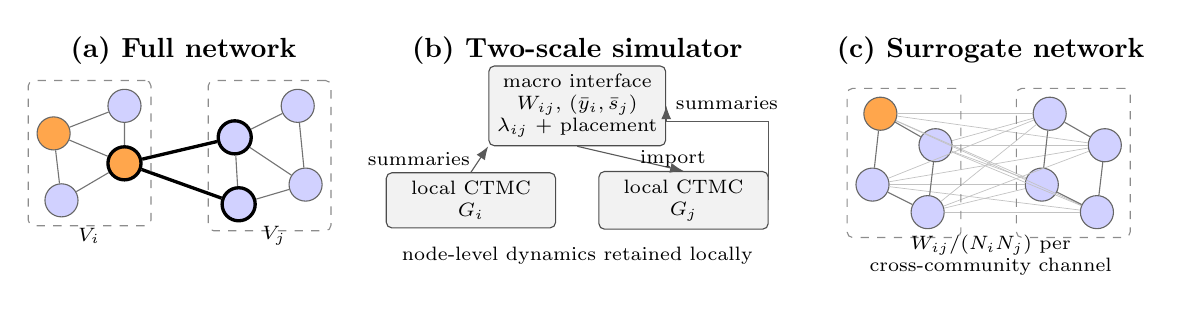
\begin{tikzpicture}[
  x=1cm,y=1cm,
  font=\scriptsize,
  >=Latex,
  person/.style={circle,draw=black!60,fill=blue!18,minimum size=4.2mm,inner sep=0pt},
  infected/.style={person,fill=orange!70},
  bridge/.style={person,very thick,draw=black},
  bridgeinf/.style={infected,very thick,draw=black},
  commbox/.style={draw=black!45,dashed,rounded corners=2pt,inner sep=3pt},
  macrobox/.style={draw=black!70,rounded corners=2pt,fill=black!5,align=center,inner sep=3pt},
  link/.style={draw=black!55},
  weak/.style={draw=black!24,line width=.25pt},
  flow/.style={-{Latex[length=1.7mm]},draw=black!65}
]
\node[font=\bfseries] at (0,2.25) {(a) Full network};
\node[infected] (a1) at (-1.65,1.20) {};
\node[person]   (a2) at (-1.55,0.35) {};
\node[bridgeinf](a3) at (-0.75,0.82) {};
\node[person]   (a4) at (-0.75,1.55) {};
\node[bridge]   (b1) at (0.65,1.15) {};
\node[person]   (b2) at (1.45,1.55) {};
\node[person]   (b3) at (1.55,0.55) {};
\node[bridge]   (b4) at (0.70,0.30) {};
\draw[link] (a1)--(a2)--(a3)--(a1) (a1)--(a4)--(a3);
\draw[link] (b1)--(b2)--(b3)--(b4)--(b1) (b1)--(b3);
\draw[very thick] (a3)--(b1);
\draw[very thick] (a3)--(b4);
\node[commbox,fit=(a1)(a2)(a3)(a4)] {};
\node[commbox,fit=(b1)(b2)(b3)(b4)] {};
\node at (-1.2,-0.10) {$V_i$};
\node at (1.15,-0.10) {$V_j$};

\node[font=\bfseries] at (5.0,2.25) {(b) Two-scale simulator};
\node[macrobox] (macro) at (5.0,1.55) {macro interface\\$W_{ij}$, $(\ibar_i,\sbar_j)$\\$\lambda_{ij}$ + placement};
\node[macrobox,minimum width=2.15cm,minimum height=.70cm] (li) at (3.65,0.35) {local CTMC\\$G_i$};
\node[macrobox,minimum width=2.15cm,minimum height=.70cm] (lj) at (6.35,0.35) {local CTMC\\$G_j$};
\draw[flow] (li.north) -- node[left] {summaries} (macro.south west);
\draw[flow] (macro.south) -- node[right] {import} (lj.north);
\draw[flow] (lj.east) -- ++(0,1.0) -| node[pos=1.08,right] {summaries} (macro.east);
\node at (5.0,-0.35) {node-level dynamics retained locally};

\node[font=\bfseries] at (10.25,2.25) {(c) Surrogate network};
\node[infected] (c1) at (8.85,1.45) {};
\node[person]   (c2) at (8.75,0.55) {};
\node[person]   (c3) at (9.55,1.05) {};
\node[person]   (c4) at (9.45,0.20) {};
\node[person]   (d1) at (11.00,1.45) {};
\node[person]   (d2) at (10.90,0.55) {};
\node[person]   (d3) at (11.70,1.05) {};
\node[person]   (d4) at (11.60,0.20) {};
\foreach \u in {c1,c2,c3,c4}{\foreach \v in {d1,d2,d3,d4}{\draw[weak] (\u)--(\v);}}
\draw[link] (c1)--(c2)--(c4)--(c3)--(c1);
\draw[link] (d1)--(d2)--(d4)--(d3)--(d1);
\node[commbox,fit=(c1)(c2)(c3)(c4)] {};
\node[commbox,fit=(d1)(d2)(d3)(d4)] {};
\node[align=center] at (10.25,-0.35) {$W_{ij}/(N_iN_j)$ per\\cross-community channel};
\end{tikzpicture}
\par\small\textbf{\textcolor{black}{Три подання зв'язку між спільнотами. (a) У повній мережі інфекція переходить лише через показані фізичні ребра та їхні вузли-мости. (b) Двомасштабний метод зберігає окремий локальний симулятор для кожної спільноти. Макрорівень отримує кількості вузлів у різних станах, використовує $W_{ij}$ для генерування міжспільнотного зараження та вибирає його ціль рівномірно серед сприйнятливих вузлів. (c) Ідеальний двомасштабний процес еквівалентний процесу на сурогатній мережі, де кожна напрямлена пара вузлів між двома спільнотами має слабкий зв'язок. Загальна вага всіх цих зв'язків дорівнює $W_{ij}$. Помаранчеві вузли --- інфіковані, сині --- сприйнятливі.}}

\end{minipage}\par
\end{minipage} &
\begin{minipage}[t]{\linewidth}
\par\noindent\begin{minipage}{\linewidth}
\color{black}\centering
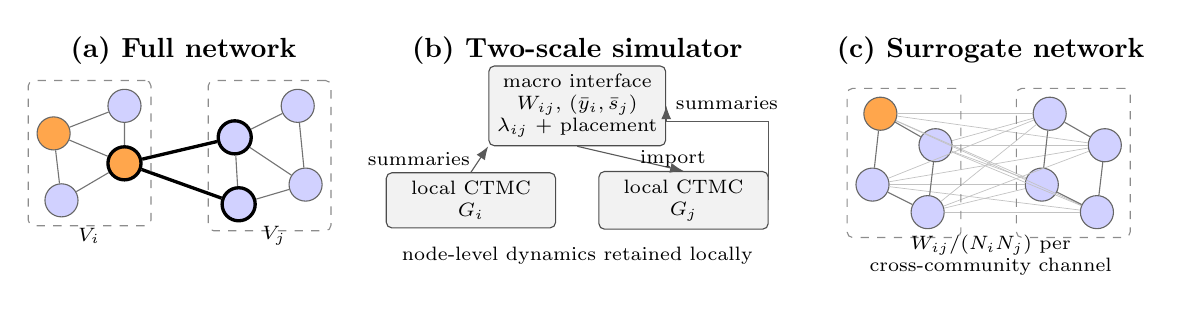
\begin{tikzpicture}[
  x=1cm,y=1cm,
  font=\scriptsize,
  >=Latex,
  person/.style={circle,draw=black!60,fill=blue!18,minimum size=4.2mm,inner sep=0pt},
  infected/.style={person,fill=orange!70},
  bridge/.style={person,very thick,draw=black},
  bridgeinf/.style={infected,very thick,draw=black},
  commbox/.style={draw=black!45,dashed,rounded corners=2pt,inner sep=3pt},
  macrobox/.style={draw=black!70,rounded corners=2pt,fill=black!5,align=center,inner sep=3pt},
  link/.style={draw=black!55},
  weak/.style={draw=black!24,line width=.25pt},
  flow/.style={-{Latex[length=1.7mm]},draw=black!65}
]
\node[font=\bfseries] at (0,2.25) {(a) Full network};
\node[infected] (a1) at (-1.65,1.20) {};
\node[person]   (a2) at (-1.55,0.35) {};
\node[bridgeinf](a3) at (-0.75,0.82) {};
\node[person]   (a4) at (-0.75,1.55) {};
\node[bridge]   (b1) at (0.65,1.15) {};
\node[person]   (b2) at (1.45,1.55) {};
\node[person]   (b3) at (1.55,0.55) {};
\node[bridge]   (b4) at (0.70,0.30) {};
\draw[link] (a1)--(a2)--(a3)--(a1) (a1)--(a4)--(a3);
\draw[link] (b1)--(b2)--(b3)--(b4)--(b1) (b1)--(b3);
\draw[very thick] (a3)--(b1);
\draw[very thick] (a3)--(b4);
\node[commbox,fit=(a1)(a2)(a3)(a4)] {};
\node[commbox,fit=(b1)(b2)(b3)(b4)] {};
\node at (-1.2,-0.10) {$V_i$};
\node at (1.15,-0.10) {$V_j$};

\node[font=\bfseries] at (5.0,2.25) {(b) Two-scale simulator};
\node[macrobox] (macro) at (5.0,1.55) {macro interface\\$W_{ij}$, $(\ibar_i,\sbar_j)$\\$\lambda_{ij}$ + placement};
\node[macrobox,minimum width=2.15cm,minimum height=.70cm] (li) at (3.65,0.35) {local CTMC\\$G_i$};
\node[macrobox,minimum width=2.15cm,minimum height=.70cm] (lj) at (6.35,0.35) {local CTMC\\$G_j$};
\draw[flow] (li.north) -- node[left] {summaries} (macro.south west);
\draw[flow] (macro.south) -- node[right] {import} (lj.north);
\draw[flow] (lj.east) -- ++(0,1.0) -| node[pos=1.08,right] {summaries} (macro.east);
\node at (5.0,-0.35) {node-level dynamics retained locally};

\node[font=\bfseries] at (10.25,2.25) {(c) Surrogate network};
\node[infected] (c1) at (8.85,1.45) {};
\node[person]   (c2) at (8.75,0.55) {};
\node[person]   (c3) at (9.55,1.05) {};
\node[person]   (c4) at (9.45,0.20) {};
\node[person]   (d1) at (11.00,1.45) {};
\node[person]   (d2) at (10.90,0.55) {};
\node[person]   (d3) at (11.70,1.05) {};
\node[person]   (d4) at (11.60,0.20) {};
\foreach \u in {c1,c2,c3,c4}{\foreach \v in {d1,d2,d3,d4}{\draw[weak] (\u)--(\v);}}
\draw[link] (c1)--(c2)--(c4)--(c3)--(c1);
\draw[link] (d1)--(d2)--(d4)--(d3)--(d1);
\node[commbox,fit=(c1)(c2)(c3)(c4)] {};
\node[commbox,fit=(d1)(d2)(d3)(d4)] {};
\node[align=center] at (10.25,-0.35) {$W_{ij}/(N_iN_j)$ per\\cross-community channel};
\end{tikzpicture}
\par\small\textbf{\textcolor{black}{Три подання зв'язку між спільнотами. (a) У повній мережі інфекція переходить лише через показані фізичні ребра та їхні вузли-мости. (b) Двомасштабний метод зберігає окремий локальний симулятор для кожної спільноти. Макрорівень отримує кількості вузлів у різних станах, використовує $W_{ij}$ для генерування міжспільнотного зараження та вибирає його ціль рівномірно серед сприйнятливих вузлів. (c) Ідеальний двомасштабний процес еквівалентний процесу на сурогатній мережі, де кожна напрямлена пара вузлів між двома спільнотами має слабкий зв'язок. Загальна вага всіх цих зв'язків дорівнює $W_{ij}$. Помаранчеві вузли --- інфіковані, сині --- сприйнятливі.}}

\end{minipage}\par
\end{minipage} \\[5mm]
\begin{minipage}[t]{\linewidth}
\subsection*{3.3. Локальні симулятори}
\end{minipage} &
\begin{minipage}[t]{\linewidth}
\subsection*{3.3. Локальні симулятори}
\end{minipage} \\[5mm]
\begin{minipage}[t]{\linewidth}
Кожна спільнота має окремий симулятор Gillespie для свого графа $G_i$. Він застосовує інтенсивності зараження та видалення з~(2), використовуючи лише локальні ребра $E_{ii}$. Реалізація оновлює лише ті інтенсивності, на які вплинула остання подія, як у \citet{kuryliak2025simulating}. Кожен локальний симулятор має власний потік випадкових чисел.
\end{minipage} &
\begin{minipage}[t]{\linewidth}
Кожна спільнота має свій симулятор Gillespie для графа $G_i$. Він моделює зараження та видалення за~(2), враховуючи лише внутрішні контакти $E_{ii}$. Після події оновлюються лише ті інтенсивності, які вона змінила, як у \citet{kuryliak2025simulating}. Кожен симулятор має власний потік випадкових чисел.
\end{minipage} \\[5mm]
\begin{minipage}[t]{\linewidth}
Макрорівень може просунути локальний симулятор до заданого часу. Симулятор виконує локальні події до цього моменту. Потім макрорівень може імпортувати інфекцію, змінивши стан вибраного сприйнятливого вузла на $I$. Це змінює локальні інтенсивності. Реалізація зберігає невикористану частину випадкового порога наступної локальної події та перераховує час очікування за новою сумарною інтенсивністю. Тип події та її вузол вибираються за оновленими інтенсивностями. Новий локальний поріг генерується лише тоді, коли збереженого порога немає. Кожен локальний годинник має власний поріг, окремий від макропорога, описаного в Розділі~3.5. За заданих часів імпорту та цільових вузлів локальний симулятор виконує правила CTMC своєї мережі. Наближення виникає через спосіб генерування імпортів і вибору їхніх цільових вузлів.
\end{minipage} &
\begin{minipage}[t]{\linewidth}
Планувальник задає час, до якого локальний симулятор має виконати свої події. У цей момент він може додати імпорт: заразити вибраний сприйнятливий вузол. Після цього локальні інтенсивності змінюються. Симулятор зберігає невикористану частину випадкового порога наступної локальної події й перераховує час очікування за новою сумарною інтенсивністю. Подію та її вузол вибирає за оновленими інтенсивностями. Новий поріг генерує лише тоді, коли збереженого немає. Локальні пороги й поріг міжспільнотної події окремі; останній описано в Розділі~3.5. За заданих часів і цілей імпорту локальний симулятор точно виконує правила своєї мережі. Похибка зв'язування спільнот залежить від того, як планувальник визначає імпорти та вибирає їхні цілі.
\end{minipage} \\[5mm]
\begin{minipage}[t]{\linewidth}
\subsection*{3.4. Макрорівень}
\end{minipage} &
\begin{minipage}[t]{\linewidth}
\subsection*{3.4. Макрорівень}
\end{minipage} \\[5mm]
\begin{minipage}[t]{\linewidth}
Макрорівень представляє спільноту її поточними частками вузлів, а напрямлений зв'язок --- вагою $W_{ij}$. Інтенсивність зараження зі спільноти $i$ до спільноти $j$:
\begin{equation*}\lambda_{ij}(t)=\beta_{\mathrm{out}}W_{ij}\ibar_i(t)\sbar_j(t),
\qquad \Theta(t)=\sum_{i\neq j}\lambda_{ij}(t).\tag{4}
\end{equation*}
Кожен множник має простий зміст. $\beta_{\mathrm{out}}W_{ij}$ задає загальну силу зв'язку; $\ibar_i$ --- частку інфікованих у спільноті-джерелі; $\sbar_j$ --- частку сприйнятливих у спільноті-одержувачі. Сума $\Theta$ --- інтенсивність будь-якого міжспільнотного зараження.
\end{minipage} &
\begin{minipage}[t]{\linewidth}
Планувальник використовує частки вузлів у різних станах і вагу $W_{ij}$. Інтенсивність передавання зі спільноти $i$ до спільноти $j$ дорівнює
\begin{equation*}\lambda_{ij}(t)=\beta_{\mathrm{out}}W_{ij}\ibar_i(t)\sbar_j(t),
\qquad \Theta(t)=\sum_{i\neq j}\lambda_{ij}(t).\tag{4}
\end{equation*}
Тут $\beta_{\mathrm{out}}W_{ij}$ задає загальну силу зв'язку, $\ibar_i$ --- частку інфікованих у джерелі, а $\sbar_j$ --- частку сприйнятливих в одержувачі. Що більше цих вузлів, то вища інтенсивність передавання. Сума $\Theta$ враховує всі напрямки між спільнотами.
\end{minipage} \\[5mm]
\begin{minipage}[t]{\linewidth}
Коли така подія відбувається, спочатку вибирають спільноту-джерело та спільноту-одержувача $(i,j)$ з імовірністю $\lambda_{ij}/\Theta$. Потім у спільноті $j$ рівномірно вибирають один сприйнятливий вузол і заражають його. Якщо таких вузлів 20, кожен має імовірність $1/20$. Вибір не враховує справжні вузли-мости, оскільки агрегований інтерфейс їх не знає. У подальших формулах цю імовірність позначаємо $\Pi_{ij}(v\mid x)=1/s_j$ для $v\in S_j$, де $x$ --- поточний стан мережі. Отже, $\Pi$ просто позначає імовірність вибору конкретного сприйнятливого вузла. Інші правила можливі, якщо є інформація про вузли-мости. Додатковий калібрувальний множник у реалізації дорівнює одиниці в усіх експериментах.
\end{minipage} &
\begin{minipage}[t]{\linewidth}
Коли така подія відбувається, спочатку вибирають спільноту-джерело та спільноту-одержувача $(i,j)$ з імовірністю $\lambda_{ij}/\Theta$. Потім у спільноті $j$ рівномірно вибирають один сприйнятливий вузол і заражають його. Якщо таких вузлів 20, кожен має імовірність $1/20$. Вибір не враховує справжні вузли-мости, оскільки агрегований інтерфейс їх не знає. У подальших формулах цю імовірність позначаємо $\Pi_{ij}(v\mid x)=1/s_j$ для $v\in S_j$, де $x$ --- поточний стан мережі. Отже, $\Pi$ просто позначає імовірність вибору конкретного сприйнятливого вузла. Інші правила можливі, якщо є інформація про вузли-мости. Додатковий калібрувальний множник у реалізації дорівнює одиниці в усіх експериментах.
\end{minipage} \\[5mm]
\begin{minipage}[t]{\linewidth}
Ця агрегована інтенсивність загалом наближено описує передавання через справжні фізичні ребра. Для заданих кількостей вузлів у станах вона дорівнює очікуваній інтенсивності за рівномірного випадкового вибору кінців ребер, перш ніж враховано їхні конкретні ідентичності, стани та історію епідемії. Це не гарантує правильної інтенсивності для вже реалізованої епідемії на конкретних ребрах. Для рівномірного зв'язку «усі з усіма» вона є фактичною інтенсивністю, як пояснено в Розділі~4. Значення $\Theta$ змінюється після локальної події або імпорту, які змінюють кількості вузлів у станах.
\end{minipage} &
\begin{minipage}[t]{\linewidth}
Формула усереднює передавання між спільнотами. За заданих кількостей інфікованих і сприйнятливих вона дорівнює очікуваній інтенсивності, якщо кінці міжспільнотних ребер вибрати рівномірно й випадково. Для конкретної мережі інтенсивність може бути іншою: важливі стани саме вузлів із міжспільнотними контактами та історія заражень. Для сурогатної мережі зі зв'язками «усі з усіма» формула точна (Розділ~4). Значення $\Theta$ оновлюється після подій, що змінюють кількості вузлів у різних станах.
\end{minipage} \\[5mm]
\begin{minipage}[t]{\linewidth}
\subsection*{3.5. Час подій та синхронізація}
\end{minipage} &
\begin{minipage}[t]{\linewidth}
\subsection*{3.5. Час подій та синхронізація}
\end{minipage} \\[5mm]
\begin{minipage}[t]{\linewidth}
Після макроподії в час $t_0$ генеруємо випадковий поріг $E\sim\Exp(1)$: експоненційне випадкове число із середнім один. Починаючи з нуля, накопичуємо загальну інтенсивність $\Theta$. Наступна макроподія відбувається в перший момент $t^\ast$, коли накопичена величина досягає $E$:
\begin{equation*}\int_{t_0}^{t^\ast}\Theta(s)\,ds=E.\tag{5}
\end{equation*}
Інакше кажучи, площа під кривою інтенсивності зростає до випадкового порога. Якщо поріг не досягнуто, наступної макроподії немає. Це стандартний спосіб визначення часу події за накопиченою інтенсивністю \citep{ethier1986,anderson2007}. За сталої $\Theta$ час очікування дорівнює $E/\Theta$. Якщо згенерувати $E=-\ln U$, де $U$ рівномірно розподілене на $(0,1)$, отримуємо звичний час очікування Gillespie. Коли локальна подія змінює $\Theta$, зберігаємо той самий поріг і продовжуємо накопичення з новою інтенсивністю. Новий макропоріг генеруємо лише після макроподії. Це той самий годинник за накопиченою інтенсивністю, який описано в конференційній роботі. Точне визначення першого досягнення порога задає ідеальний процес; описаний нижче розрахунок на часовій сітці наближено визначає цей момент. У Розділі~4.1 показано, що ідеальний процес точний для сурогатної мережі.
\end{minipage} &
\begin{minipage}[t]{\linewidth}
Після міжспільнотного зараження в час $t_0$ генеруємо випадковий поріг $E\sim\Exp(1)$ --- експоненційне число із середнім один. Від цього моменту накопичуємо загальну інтенсивність $\Theta$. Наступне міжспільнотне зараження відбувається в перший момент $t^\ast$, коли накопичена величина досягає порога:
\begin{equation*}\int_{t_0}^{t^\ast}\Theta(s)\,ds=E.\tag{5}
\end{equation*}
Інтеграл --- це площа під кривою інтенсивності. Вона зростає до порога $E$; якщо його не досягнуто, подія не відбувається. Так визначають час події за змінної інтенсивності \citep{ethier1986,anderson2007}. За сталої $\Theta$ час очікування дорівнює $E/\Theta$. Якщо взяти $E=-\ln U$, де $U$ рівномірно розподілене на $(0,1)$, отримуємо звичну формулу Gillespie. Коли локальна подія змінює $\Theta$, зберігаємо поріг і вже накопичену величину, а далі додаємо внесок нової інтенсивності. Новий поріг генеруємо після міжспільнотного зараження. Цей принцип використано і в конференційній роботі. Ідеальний процес визначає момент досягнення порога точно; наша реалізація оцінює його за часовою сіткою. Ідеальний процес точний для сурогатної мережі (Розділ~4.1).
\end{minipage} \\[5mm]
\begin{minipage}[t]{\linewidth}
Реалізований планувальник узгоджує локальні симулятори на інтервалах довжини $\tau$. У конференційному описі цього годинника також використано оцінку інтенсивності в середині кроку. Тут уточнюємо, як отримати її від локальних симуляторів. Нехай $A$ --- уже накопичена величина від попередньої макроподії. Для поточного інтервалу $[t,t_g)$ копіюємо кожен локальний симулятор разом зі станом генератора випадкових чисел і просуваємо копію до середини інтервалу. За копіями обчислюємо оцінку загальної макроінтенсивності $\Theta_{\mathrm{mid}}$. Оцінений приріст за залишок інтервалу дорівнює $\Theta_{\mathrm{mid}}(t_g-t)$. Якщо $A$ плюс цей приріст менше за $E$ (випадковий макропоріг), справжні симулятори просуваються до $t_g$. Інакше час події оцінюємо як
\begin{equation*}t^\ast=t+\frac{E-A}{\Theta_{\mathrm{mid}}}.\tag{6}
\end{equation*}
Тут $E$ --- випадковий макропоріг, а $A$ --- уже накопичена до нього величина. Чисельник $E-A$ --- залишок до порога; ділення на оцінену інтенсивність дає залишковий час очікування. Наприклад, за $E=1$, $A=0.4$ та $\Theta_{\mathrm{mid}}=0.2$ оцінений час очікування дорівнює трьом одиницям часу. Планувальник просуває справжні симулятори до $t^\ast$, за їхніми станами в цей момент вибирає спільноту-джерело та спільноту-одержувача, вибирає сприйнятливий цільовий вузол і застосовує зараження. Повну послідовність наведено в Алгоритмі~1.
\end{minipage} &
\begin{minipage}[t]{\linewidth}
У реалізації час поділено на інтервали довжини $\tau$. Час міжспільнотного зараження може лежати всередині інтервалу: його не округлюють до точки сітки. Для оцінки використовуємо інтенсивність у середині інтервалу, як у конференційному описі. Позначимо через $A$ уже накопичену величину. На поточному інтервалі $[t,t_g)$ копіюємо локальні симулятори разом зі станами їхніх генераторів випадкових чисел. Копії виконуємо до середини інтервалу й за їхніми станами обчислюємо $\Theta_{\mathrm{mid}}$. Оцінка приросту дорівнює $\Theta_{\mathrm{mid}}(t_g-t)$. Якщо $A$ разом із цим приростом ще менше за $E$, справжні симулятори виконуються до $t_g$. Інакше оцінюємо час зараження:
\begin{equation*}t^\ast=t+\frac{E-A}{\Theta_{\mathrm{mid}}}.\tag{6}
\end{equation*}
Залишок до порога дорівнює $E-A$. Ділення на оцінену інтенсивність дає час, потрібний для його накопичення. Наприклад, якщо $E=1$, $A=0.4$ і $\Theta_{\mathrm{mid}}=0.2$, час очікування дорівнює трьом одиницям часу. Планувальник виконує справжні симулятори до $t^\ast$ і за їхніми станами вибирає напрямок передавання та сприйнятливий вузол-одержувач. Потім заражає цей вузол. Повну послідовність наведено в Алгоритмі~1.
\end{minipage} \\[5mm]
\begin{minipage}[t]{\linewidth}
\par\noindent\begin{minipage}{\linewidth}
\color{black}
\par\small\textbf{\textcolor{black}{Один запуск двомасштабного симулятора з узгодженням за часовою сіткою.}}

\small
\fbox{\begin{minipage}{0.94\linewidth}
\textbf{Вхід:} локальні графи $G_i$, ваги $W_{ij}$, інтенсивності, крок $\tau$, горизонт $T_{\mathrm{end}}$ та початковий стан.
\begin{enumerate}
\item Установити $t=0$ і $A=0$; згенерувати $E\sim\Exp(1)$.
\item Поки $t<T_{\mathrm{end}}$ й інфекція може поширюватися, встановити $t_g=\min(t+\tau,T_{\mathrm{end}})$ та обробити інтервал до $t_g$.
\item Скопіювати кожен локальний симулятор разом зі станом генератора випадкових чисел. Просунути копії до середини залишку інтервалу та обчислити $\Theta_{\mathrm{mid}}$ за~(4).
\item Якщо $A+\Theta_{\mathrm{mid}}(t_g-t)<E$, просунути справжні симулятори до $t_g$, додати цю величину до $A$, встановити $t=t_g$ і повернутися до кроку 2.
\item Інакше обчислити $t^\ast$ за~(6) та просунути справжні симулятори до $t^\ast$.
\item Вибрати $(i,j)$ з імовірністю $\lambda_{ij}(t^\ast)/\Theta(t^\ast)$. Рівномірно вибрати $v$ з $S_j(t^\ast)$ та імпортувати зараження у $v$. Оновити локальний симулятор одержувача, зберігаючи невикористаний експоненційний поріг і вибираючи локальну подію за новими інтенсивностями.
\item Установити $t=t^\ast$ і $A=0$, згенерувати нове $E\sim\Exp(1)$ та так само обробити залишок поточного інтервалу.
\end{enumerate}
\end{minipage}}
\end{minipage}\par
\end{minipage} &
\begin{minipage}[t]{\linewidth}
\par\noindent\begin{minipage}{\linewidth}
\color{black}
\par\small\textbf{\textcolor{black}{Один запуск двомасштабного симулятора з узгодженням за часовою сіткою.}}

\small
\fbox{\begin{minipage}{0.94\linewidth}
\textbf{Вхід:} локальні графи $G_i$, ваги $W_{ij}$, інтенсивності, крок $\tau$, горизонт $T_{\mathrm{end}}$ та початковий стан.
\begin{enumerate}
\item Установити $t=0$ і $A=0$; згенерувати $E\sim\Exp(1)$.
\item Поки $t<T_{\mathrm{end}}$ й інфекція може поширюватися, встановити $t_g=\min(t+\tau,T_{\mathrm{end}})$ та обробити інтервал до $t_g$.
\item Скопіювати кожен локальний симулятор разом зі станом генератора випадкових чисел. Просунути копії до середини залишку інтервалу та обчислити $\Theta_{\mathrm{mid}}$ за~(4).
\item Якщо $A+\Theta_{\mathrm{mid}}(t_g-t)<E$, просунути справжні симулятори до $t_g$, додати цю величину до $A$, встановити $t=t_g$ і повернутися до кроку 2.
\item Інакше обчислити $t^\ast$ за~(6) та просунути справжні симулятори до $t^\ast$.
\item Вибрати $(i,j)$ з імовірністю $\lambda_{ij}(t^\ast)/\Theta(t^\ast)$. Рівномірно вибрати $v$ з $S_j(t^\ast)$ та імпортувати зараження у $v$. Оновити локальний симулятор одержувача, зберігаючи невикористаний експоненційний поріг і вибираючи локальну подію за новими інтенсивностями.
\item Установити $t=t^\ast$ і $A=0$, згенерувати нове $E\sim\Exp(1)$ та так само обробити залишок поточного інтервалу.
\end{enumerate}
\end{minipage}}
\end{minipage}\par
\end{minipage} \\[5mm]
\begin{minipage}[t]{\linewidth}
Копіювання станів генераторів випадкових чисел важливе: якщо до середини інтервалу не відбудеться імпорт, копія відтворить ту саму траєкторію, що й справжній симулятор. Оцінка середньої точки точна на інтервалі без локальних подій. Її похибка визначення часу та використання майбутнього стану не більш як на $\tau/2$ зникають зі зменшенням $\tau$ до нуля.
\end{minipage} &
\begin{minipage}[t]{\linewidth}
Копії використовують той самий стан генератора випадкових чисел, що й справжні симулятори. Тому до першого імпорту вони відтворюють ту саму локальну траєкторію. Якщо на інтервалі немає локальних подій, інтенсивність стала й оцінка за серединою інтервалу точна. Якщо такі події є, оцінка може використати стан, пізніший за оцінений час імпорту, не більш ніж на $\tau/2$. Менший крок зменшує цей часовий зсув; у границі $\tau\to0$ похибка сітки зникає.
\end{minipage} \\[5mm]
\begin{minipage}[t]{\linewidth}
Часова сітка потрібна, оскільки планувальник працює з локальними симуляторами як із «чорними скриньками». Якщо вони також повідомляють часи наступних локальних подій, планувальник може об'єднати ці часи та точно накопичувати $\Theta$, яка стала між подіями. Такий подієвий варіант усуває чисельну похибку синхронізації. В експериментах цієї статті використано реалізований сітковий варіант із $\tau=1$.
\end{minipage} &
\begin{minipage}[t]{\linewidth}
Щоб обійтися без часової сітки, локальні симулятори мають повідомляти часи своїх наступних подій. Тоді планувальник може обробляти події в часовому порядку й точно накопичувати $\Theta$, яка стала між подіями. Імпорт застосовується в момент його виникнення, після чого локальні інтенсивності оновлюються. Такий варіант усуває похибку часової синхронізації, але зберігає усереднений опис міжспільнотних зв'язків. В експериментах використано варіант із часовою сіткою та кроком $\tau=1$.
\end{minipage} \\[5mm]
\begin{minipage}[t]{\linewidth}
\subsection*{3.6. Обчислювальна структура та застосування}
\end{minipage} &
\begin{minipage}[t]{\linewidth}
\subsection*{3.6. Обчислювальна структура та застосування}
\end{minipage} \\[5mm]
\begin{minipage}[t]{\linewidth}
\Full{} зберігає всі локальні та міжспільнотні канали, а обсяг роботи на одну подію зростає зі степенем вузла \citep{kuryliak2025simulating}. \TS{} зберігає локальні графи та матрицю загальних ваг розміру $M\times M$. У конференційній роботі обговорено таке скорочення даних про міжспільнотні контакти \citep{kuryliak2025towards}. Його значення залежить від задачі. Заміна багатьох індивідуальних міжспільнотних ребер однією вагою може зменшити обсяг збережених даних. Якщо таких ребер лише кілька, економія може бути малою; локальні графи все одно потрібно зберігати.
\end{minipage} &
\begin{minipage}[t]{\linewidth}
\Full{} зберігає всі контакти, зокрема між спільнотами. Обсяг роботи після події залежить від кількості сусідів відповідного вузла \citep{kuryliak2025simulating}. \TS{} зберігає локальні графи та матрицю міжспільнотних ваг розміру $M\times M$. Таке скорочення даних обговорено в конференційній роботі \citep{kuryliak2025towards}. Якщо міжспільнотних ребер багато, заміна їх загальними вагами може зменшити обсяг даних. Якщо ребер мало, економія може бути незначною. Локальні графи в будь-якому разі потрібно зберігати.
\end{minipage} \\[5mm]
\begin{minipage}[t]{\linewidth}
Окремі локальні симулятори також створюють можливість паралельного виконання. Коли планувальник визначив наступний цільовий час ($t_g$ або $t^\ast$), локальні симулятори можна незалежно просунути до цього самого часу. Копії для оцінки середньої точки також можна обробляти паралельно. Потім макрорівень має зібрати кількості вузлів і застосувати імпорт, якщо він запланований, перш ніж продовжувати. У досліджуваній реалізації локальні симулятори просуваються послідовно; паралельне виконання в межах одного запуску є можливим розширенням, а не виміряним прискоренням. Локальні симулятори також можуть мати різні налаштування для різних спільнот.
\end{minipage} &
\begin{minipage}[t]{\linewidth}
Локальні симулятори можна виконувати паралельно до спільного часу $t_g$ або $t^\ast$, який уже визначив планувальник. Копії для оцінки інтенсивності також можна виконувати паралельно. Потім потрібно зібрати стани спільнот і застосувати імпорт, якщо він має відбутися. У нашій реалізації локальні симулятори виконуються послідовно; можливе паралельне виконання ще не дає підстав заявляти про прискорення. Для різних спільнот також можна задавати різні локальні налаштування.
\end{minipage} \\[5mm]
\begin{minipage}[t]{\linewidth}
Сітковий планувальник додає роботу через копіювання локальних станів та узгодження спільнот. Тому ні менше використання пам'яті, ні швидше виконання не гарантовані. Метод корисний, коли конкретні міжспільнотні контакти недоступні або надто численні для явного подання. Виміряний час виконання наведено в Розділі~7.2; головний предмет цієї статті --- похибка наближення.
\end{minipage} &
\begin{minipage}[t]{\linewidth}
Копіювання станів і синхронізація потребують додаткової роботи, тому метод не гарантує меншого використання пам'яті або швидшого виконання. Його можна застосовувати, коли конкретні міжспільнотні контакти невідомі або їх надто багато для явного зберігання. Час виконання наведено в Розділі~7.2. Основне питання цієї статті --- точність такого спрощення.
\end{minipage} \\[5mm]
\end{longtable}
\clearpage
\section*{Література (спільна для обох колонок)}
\begin{thebibliography}{26}
\expandafter\ifx\csname natexlab\endcsname\relax\def\natexlab#1{#1}\fi
\providecommand{\url}[1]{\texttt{#1}}
\providecommand{\href}[2]{#2}
\providecommand{\path}[1]{#1}
\providecommand{\DOIprefix}{doi:}
\providecommand{\ArXivprefix}{arXiv:}
\providecommand{\URLprefix}{URL: }
\providecommand{\Pubmedprefix}{pmid:}
\providecommand{\doi}[1]{\href{http://dx.doi.org/#1}{\path{#1}}}
\providecommand{\Pubmed}[1]{\href{pmid:#1}{\path{#1}}}
\providecommand{\bibinfo}[2]{#2}
\ifx\xfnm\relax \def\xfnm[#1]{\unskip,\space#1}\fi
%Type = Article
\bibitem[{Ajelli et~al.(2010)Ajelli, Gon{\c{c}}alves, Balcan, Colizza, Hu,
  Ramasco, Merler and Vespignani}]{ajelli2010}
\bibinfo{author}{Ajelli, M.}, \bibinfo{author}{Gon{\c{c}}alves, B.},
  \bibinfo{author}{Balcan, D.}, \bibinfo{author}{Colizza, V.},
  \bibinfo{author}{Hu, H.}, \bibinfo{author}{Ramasco, J.J.},
  \bibinfo{author}{Merler, S.}, \bibinfo{author}{Vespignani, A.},
  \bibinfo{year}{2010}.
\newblock \bibinfo{title}{Comparing large-scale computational approaches to
  epidemic modeling: Agent-based versus structured metapopulation models}.
\newblock \bibinfo{journal}{BMC Infectious Diseases} \bibinfo{volume}{10},
  \bibinfo{pages}{190}.
\newblock \DOIprefix\doi{10.1186/1471-2334-10-190}.
%Type = Article
\bibitem[{Anderson(2007)}]{anderson2007}
\bibinfo{author}{Anderson, D.F.}, \bibinfo{year}{2007}.
\newblock \bibinfo{title}{A modified next reaction method for simulating
  chemical systems with time dependent propensities and delays}.
\newblock \bibinfo{journal}{The Journal of Chemical Physics}
  \bibinfo{volume}{127}, \bibinfo{pages}{214107}.
\newblock \DOIprefix\doi{10.1063/1.2799998}.
%Type = Article
\bibitem[{Balcan et~al.(2009)Balcan, Colizza, Gon{\c{c}}alves, Hu, Ramasco and
  Vespignani}]{balcan2009}
\bibinfo{author}{Balcan, D.}, \bibinfo{author}{Colizza, V.},
  \bibinfo{author}{Gon{\c{c}}alves, B.}, \bibinfo{author}{Hu, H.},
  \bibinfo{author}{Ramasco, J.J.}, \bibinfo{author}{Vespignani, A.},
  \bibinfo{year}{2009}.
\newblock \bibinfo{title}{Multiscale mobility networks and the spatial
  spreading of infectious diseases}.
\newblock \bibinfo{journal}{Proceedings of the National Academy of Sciences}
  \bibinfo{volume}{106}, \bibinfo{pages}{21484--21489}.
\newblock \DOIprefix\doi{10.1073/pnas.0906910106}.
%Type = Article
\bibitem[{Balcan et~al.(2010)Balcan, Colizza, Gon{\c{c}}alves, Hu, Ramasco and
  Vespignani}]{balcan2010modeling}
\bibinfo{author}{Balcan, D.}, \bibinfo{author}{Colizza, V.},
  \bibinfo{author}{Gon{\c{c}}alves, B.}, \bibinfo{author}{Hu, H.},
  \bibinfo{author}{Ramasco, J.J.}, \bibinfo{author}{Vespignani, A.},
  \bibinfo{year}{2010}.
\newblock \bibinfo{title}{Modeling the spatial spread of infectious diseases:
  The global epidemic and mobility computational model}.
\newblock \bibinfo{journal}{Journal of Computational Science}
  \bibinfo{volume}{1}, \bibinfo{pages}{132--145}.
\newblock \DOIprefix\doi{10.1016/j.jocs.2010.07.002}.
%Type = Article
\bibitem[{Ball et~al.(1997)Ball, Mollison and Scalia-Tomba}]{ball1997}
\bibinfo{author}{Ball, F.}, \bibinfo{author}{Mollison, D.},
  \bibinfo{author}{Scalia-Tomba, G.}, \bibinfo{year}{1997}.
\newblock \bibinfo{title}{Epidemics with two levels of mixing}.
\newblock \bibinfo{journal}{The Annals of Applied Probability}
  \bibinfo{volume}{7}, \bibinfo{pages}{46--89}.
%Type = Article
\bibitem[{Barbosa et~al.(2018)Barbosa, Barthelemy, Ghoshal, James, Lenormand,
  Louail, Menezes, Ramasco, Simini and Tomasini}]{barbosa2018human}
\bibinfo{author}{Barbosa, H.}, \bibinfo{author}{Barthelemy, M.},
  \bibinfo{author}{Ghoshal, G.}, \bibinfo{author}{James, C.R.},
  \bibinfo{author}{Lenormand, M.}, \bibinfo{author}{Louail, T.},
  \bibinfo{author}{Menezes, R.}, \bibinfo{author}{Ramasco, J.J.},
  \bibinfo{author}{Simini, F.}, \bibinfo{author}{Tomasini, M.},
  \bibinfo{year}{2018}.
\newblock \bibinfo{title}{Human mobility: Models and applications}.
\newblock \bibinfo{journal}{Physics Reports} \bibinfo{volume}{734},
  \bibinfo{pages}{1--74}.
\newblock \DOIprefix\doi{10.1016/j.physrep.2018.01.001}.
%Type = Article
\bibitem[{del Barrio et~al.(1999)del Barrio, Gin{\'e} and
  Matr{\'a}n}]{delbarrio1999}
\bibinfo{author}{del Barrio, E.}, \bibinfo{author}{Gin{\'e}, E.},
  \bibinfo{author}{Matr{\'a}n, C.}, \bibinfo{year}{1999}.
\newblock \bibinfo{title}{Central limit theorems for the {W}asserstein distance
  between the empirical and the true distributions}.
\newblock \bibinfo{journal}{The Annals of Probability} \bibinfo{volume}{27},
  \bibinfo{pages}{1009--1071}.
%Type = Article
\bibitem[{Cao et~al.(2005)Cao, Gillespie and Petzold}]{cao2005slow}
\bibinfo{author}{Cao, Y.}, \bibinfo{author}{Gillespie, D.T.},
  \bibinfo{author}{Petzold, L.R.}, \bibinfo{year}{2005}.
\newblock \bibinfo{title}{The slow-scale stochastic simulation algorithm}.
\newblock \bibinfo{journal}{The Journal of Chemical Physics}
  \bibinfo{volume}{122}, \bibinfo{pages}{014116}.
%Type = Article
\bibitem[{Chang et~al.(2021)Chang, Pierson, Koh, Gerardin, Redbird, Grusky and
  Leskovec}]{chang2021}
\bibinfo{author}{Chang, S.}, \bibinfo{author}{Pierson, E.},
  \bibinfo{author}{Koh, P.W.}, \bibinfo{author}{Gerardin, J.},
  \bibinfo{author}{Redbird, B.}, \bibinfo{author}{Grusky, D.},
  \bibinfo{author}{Leskovec, J.}, \bibinfo{year}{2021}.
\newblock \bibinfo{title}{Mobility network models of {COVID-19} explain
  inequities and inform reopening}.
\newblock \bibinfo{journal}{Nature} \bibinfo{volume}{589},
  \bibinfo{pages}{82--87}.
\newblock \DOIprefix\doi{10.1038/s41586-020-2923-3}.
%Type = Article
\bibitem[{Colizza et~al.(2007)Colizza, Pastor-Satorras and
  Vespignani}]{colizza2007reaction}
\bibinfo{author}{Colizza, V.}, \bibinfo{author}{Pastor-Satorras, R.},
  \bibinfo{author}{Vespignani, A.}, \bibinfo{year}{2007}.
\newblock \bibinfo{title}{Reaction--diffusion processes and metapopulation
  models in heterogeneous networks}.
\newblock \bibinfo{journal}{Nature Physics} \bibinfo{volume}{3},
  \bibinfo{pages}{276--282}.
\newblock \DOIprefix\doi{10.1038/nphys560}.
%Type = Article
\bibitem[{Colizza and Vespignani(2008)}]{colizza2008}
\bibinfo{author}{Colizza, V.}, \bibinfo{author}{Vespignani, A.},
  \bibinfo{year}{2008}.
\newblock \bibinfo{title}{Epidemic modeling in metapopulation systems with
  heterogeneous coupling pattern: Theory and simulations}.
\newblock \bibinfo{journal}{Journal of Theoretical Biology}
  \bibinfo{volume}{251}, \bibinfo{pages}{450--467}.
\newblock \DOIprefix\doi{10.1016/j.jtbi.2007.11.028}.
%Type = Article
\bibitem[{Danon et~al.(2011)Danon, Ford, House, Jewell, Keeling, Roberts, Ross
  and Vernon}]{danon2011}
\bibinfo{author}{Danon, L.}, \bibinfo{author}{Ford, A.P.},
  \bibinfo{author}{House, T.}, \bibinfo{author}{Jewell, C.P.},
  \bibinfo{author}{Keeling, M.J.}, \bibinfo{author}{Roberts, G.O.},
  \bibinfo{author}{Ross, J.V.}, \bibinfo{author}{Vernon, M.C.},
  \bibinfo{year}{2011}.
\newblock \bibinfo{title}{Networks and the epidemiology of infectious disease}.
\newblock \bibinfo{journal}{Interdisciplinary Perspectives on Infectious
  Diseases} \bibinfo{volume}{2011}, \bibinfo{pages}{284909}.
\newblock \DOIprefix\doi{10.1155/2011/284909}.
%Type = Book
\bibitem[{Ethier and Kurtz(1986)}]{ethier1986}
\bibinfo{author}{Ethier, S.N.}, \bibinfo{author}{Kurtz, T.G.},
  \bibinfo{year}{1986}.
\newblock \bibinfo{title}{Markov Processes: Characterization and Convergence}.
\newblock \bibinfo{publisher}{Wiley}, \bibinfo{address}{New York}.
%Type = Article
\bibitem[{Eubank et~al.(2004)Eubank, Guclu, Kumar, Marathe, Srinivasan,
  Toroczkai and Wang}]{eubank2004}
\bibinfo{author}{Eubank, S.}, \bibinfo{author}{Guclu, H.},
  \bibinfo{author}{Kumar, V.S.A.}, \bibinfo{author}{Marathe, M.V.},
  \bibinfo{author}{Srinivasan, A.}, \bibinfo{author}{Toroczkai, Z.},
  \bibinfo{author}{Wang, N.}, \bibinfo{year}{2004}.
\newblock \bibinfo{title}{Modelling disease outbreaks in realistic urban social
  networks}.
\newblock \bibinfo{journal}{Nature} \bibinfo{volume}{429},
  \bibinfo{pages}{180--184}.
\newblock \DOIprefix\doi{10.1038/nature02541}.
%Type = Article
\bibitem[{Gibson and Bruck(2000)}]{gibson2000}
\bibinfo{author}{Gibson, M.A.}, \bibinfo{author}{Bruck, J.},
  \bibinfo{year}{2000}.
\newblock \bibinfo{title}{Efficient exact stochastic simulation of chemical
  systems with many species and many channels}.
\newblock \bibinfo{journal}{The Journal of Physical Chemistry A}
  \bibinfo{volume}{104}, \bibinfo{pages}{1876--1889}.
%Type = Article
\bibitem[{Gillespie(1977)}]{gillespie1977exact}
\bibinfo{author}{Gillespie, D.T.}, \bibinfo{year}{1977}.
\newblock \bibinfo{title}{Exact stochastic simulation of coupled chemical
  reactions}.
\newblock \bibinfo{journal}{The Journal of Physical Chemistry}
  \bibinfo{volume}{81}, \bibinfo{pages}{2340--2361}.
\newblock \DOIprefix\doi{10.1021/j100540a008}.
%Type = Article
\bibitem[{Gomes et~al.(2018)Gomes, Thule, Broman, Larsen and
  Vangheluwe}]{gomes2018cosim}
\bibinfo{author}{Gomes, C.}, \bibinfo{author}{Thule, C.},
  \bibinfo{author}{Broman, D.}, \bibinfo{author}{Larsen, P.G.},
  \bibinfo{author}{Vangheluwe, H.}, \bibinfo{year}{2018}.
\newblock \bibinfo{title}{Co-simulation: A survey}.
\newblock \bibinfo{journal}{ACM Computing Surveys} \bibinfo{volume}{51},
  \bibinfo{pages}{49:1--49:33}.
%Type = Article
\bibitem[{Haseltine and Rawlings(2002)}]{haseltine2002}
\bibinfo{author}{Haseltine, E.L.}, \bibinfo{author}{Rawlings, J.B.},
  \bibinfo{year}{2002}.
\newblock \bibinfo{title}{Approximate simulation of coupled fast and slow
  reactions for stochastic chemical kinetics}.
\newblock \bibinfo{journal}{The Journal of Chemical Physics}
  \bibinfo{volume}{117}, \bibinfo{pages}{6959--6969}.
%Type = Article
\bibitem[{Keeling and Eames(2005)}]{keeling2005}
\bibinfo{author}{Keeling, M.J.}, \bibinfo{author}{Eames, K.T.D.},
  \bibinfo{year}{2005}.
\newblock \bibinfo{title}{Networks and epidemic models}.
\newblock \bibinfo{journal}{Journal of The Royal Society Interface}
  \bibinfo{volume}{2}, \bibinfo{pages}{295--307}.
\newblock \DOIprefix\doi{10.1098/rsif.2005.0051}.
%Type = Article
\bibitem[{Kerr et~al.(2021)Kerr, Stuart, Mistry, Abeysuriya, Rosenfeld, Hart,
  N{\'u}{\~n}ez, Cohen, Selvaraj, Hagedorn, George, Jastrzebski, Izzo, Fowler,
  Palmer, Delport, Scott, Kelly, Bennette, Wagner, Chang, Oron, Wenger,
  Panovska-Griffiths, Famulare and Klein}]{kerr2021}
\bibinfo{author}{Kerr, C.C.}, \bibinfo{author}{Stuart, R.M.},
  \bibinfo{author}{Mistry, D.}, \bibinfo{author}{Abeysuriya, R.G.},
  \bibinfo{author}{Rosenfeld, K.}, \bibinfo{author}{Hart, G.R.},
  \bibinfo{author}{N{\'u}{\~n}ez, R.C.}, \bibinfo{author}{Cohen, J.A.},
  \bibinfo{author}{Selvaraj, P.}, \bibinfo{author}{Hagedorn, B.},
  \bibinfo{author}{George, L.}, \bibinfo{author}{Jastrzebski, M.},
  \bibinfo{author}{Izzo, A.S.}, \bibinfo{author}{Fowler, G.},
  \bibinfo{author}{Palmer, A.}, \bibinfo{author}{Delport, D.},
  \bibinfo{author}{Scott, N.}, \bibinfo{author}{Kelly, S.L.},
  \bibinfo{author}{Bennette, C.S.}, \bibinfo{author}{Wagner, B.G.},
  \bibinfo{author}{Chang, S.T.}, \bibinfo{author}{Oron, A.P.},
  \bibinfo{author}{Wenger, E.A.}, \bibinfo{author}{Panovska-Griffiths, J.},
  \bibinfo{author}{Famulare, M.}, \bibinfo{author}{Klein, D.J.},
  \bibinfo{year}{2021}.
\newblock \bibinfo{title}{Covasim: An agent-based model of {COVID-19} dynamics
  and interventions}.
\newblock \bibinfo{journal}{PLoS Computational Biology} \bibinfo{volume}{17},
  \bibinfo{pages}{e1009149}.
\newblock \DOIprefix\doi{10.1371/journal.pcbi.1009149}.
%Type = Book
\bibitem[{Kiss et~al.(2017)Kiss, Miller and Simon}]{kiss2017}
\bibinfo{author}{Kiss, I.Z.}, \bibinfo{author}{Miller, J.C.},
  \bibinfo{author}{Simon, P.L.}, \bibinfo{year}{2017}.
\newblock \bibinfo{title}{Mathematics of Epidemics on Networks: From Exact to
  Approximate Models}.
\newblock \bibinfo{publisher}{Springer}, \bibinfo{address}{Cham}.
\newblock \DOIprefix\doi{10.1007/978-3-319-50806-1}.
%Type = Inproceedings
\bibitem[{Kuryliak and Emmerich(2025)}]{kuryliak2025towards}
\bibinfo{author}{Kuryliak, Y.}, \bibinfo{author}{Emmerich, M.},
  \bibinfo{year}{2025}.
\newblock \bibinfo{title}{Towards complexity reduction of large-scale epidemic
  simulation in two-scale networks}, in: \bibinfo{booktitle}{Proceedings of the
  Modern Machine Learning Technologies Workshop (MoMLeT 2025)}, pp.
  \bibinfo{pages}{327--336}.
\newblock \URLprefix \url{https://ceur-ws.org/Vol-4004/}.
%Type = Article
\bibitem[{Kuryliak et~al.(2025)Kuryliak, Emmerich and
  Dosyn}]{kuryliak2025simulating}
\bibinfo{author}{Kuryliak, Y.}, \bibinfo{author}{Emmerich, M.T.M.},
  \bibinfo{author}{Dosyn, D.}, \bibinfo{year}{2025}.
\newblock \bibinfo{title}{Simulating epidemic peak dynamics on complex networks
  using efficient gillespie algorithms}.
\newblock \bibinfo{journal}{Infection, Genetics and Evolution}
  \bibinfo{volume}{132}, \bibinfo{pages}{105768}.
\newblock \DOIprefix\doi{10.1016/j.meegid.2025.105768}.
%Type = Article
\bibitem[{Pastor-Satorras et~al.(2015)Pastor-Satorras, Castellano, Van~Mieghem
  and Vespignani}]{pastorsatorras2015}
\bibinfo{author}{Pastor-Satorras, R.}, \bibinfo{author}{Castellano, C.},
  \bibinfo{author}{Van~Mieghem, P.}, \bibinfo{author}{Vespignani, A.},
  \bibinfo{year}{2015}.
\newblock \bibinfo{title}{Epidemic processes in complex networks}.
\newblock \bibinfo{journal}{Reviews of Modern Physics} \bibinfo{volume}{87},
  \bibinfo{pages}{925--979}.
\newblock \DOIprefix\doi{10.1103/RevModPhys.87.925}.
%Type = Book
\bibitem[{Shaked and Shanthikumar(2007)}]{shaked2007}
\bibinfo{author}{Shaked, M.}, \bibinfo{author}{Shanthikumar, J.G.},
  \bibinfo{year}{2007}.
\newblock \bibinfo{title}{Stochastic Orders}.
\newblock \bibinfo{publisher}{Springer}, \bibinfo{address}{New York}.
%Type = Article
\bibitem[{Vestergaard and G{\'e}nois(2015)}]{vestergaard2015}
\bibinfo{author}{Vestergaard, C.L.}, \bibinfo{author}{G{\'e}nois, M.},
  \bibinfo{year}{2015}.
\newblock \bibinfo{title}{Temporal gillespie algorithm: Fast simulation of
  contagion processes on time-varying networks}.
\newblock \bibinfo{journal}{PLoS Computational Biology} \bibinfo{volume}{11},
  \bibinfo{pages}{e1004579}.
\newblock \DOIprefix\doi{10.1371/journal.pcbi.1004579}.

\end{thebibliography}

\end{document}
